% Компиляция: pdflatex algorithm.tex  (дважды, для ссылок)
% Требует рисунки из docs/figures/ (сгенерировать: python docs/make_figures.py)
\documentclass[12pt,a4paper]{article}

\usepackage[T2A]{fontenc}
\usepackage[utf8]{inputenc}
\usepackage[russian]{babel}
\usepackage{amsmath,amssymb}
\usepackage{graphicx}
\usepackage{booktabs}
\usepackage{geometry}
\geometry{margin=25mm}
\usepackage{tikz}
\usetikzlibrary{arrows.meta,positioning,shapes.geometric,fit,backgrounds}
\usepackage[hidelinks]{hyperref}

\graphicspath{{figures/}}

\title{Алгоритм управления двухзвенным манипулятором\\
с компенсацией упругой деформации звеньев\\
по обратной связи момента приводов}
\author{}
\date{}

\usepackage{textcomp}
\newcommand{\mm}{\,\text{мм}}
\newcommand{\permil}{\text{\textperthousand}}
\newcommand{\dir}{\mathrm{dir}}

\begin{document}
\maketitle

\begin{abstract}
Рассматривается система управления плоским двухзвенным манипулятором (плечо и
предплечье) с сервоприводами HCFA~Y7 и волновыми редукторами, управляемыми по
шине EtherCAT. Особенность системы — компенсация упругой деформации звеньев и
редукторов под действием силы тяжести и полезной нагрузки при наличии
\emph{только} моторного энкодера: деформация не измеряется, а оценивается по
модели, входом для которой служит обратная связь по моменту двигателя. Приведены
кинематика, преобразование суставных координат, планирование траектории,
устранение трения волнового редуктора двунаправленным усреднением, идентификация
модели статической нагрузки и эффективной жёсткости, а также упреждающая
компенсация деформации. Дан экспериментальный материал, полученный на стенде.
\end{abstract}

\tableofcontents

\section{Постановка задачи и архитектура}

Система решает задачу позиционирования рабочего органа в декартовых координатах
$(x,z)$ в вертикальной плоскости. Цепочка преобразований:
\[
(x,z)\xrightarrow{\text{ОК}} q_\text{ц}
\xrightarrow{\text{комп.}} q_\text{кмд}
\xrightarrow{\text{joint\_map}} \text{отсчёты}
\xrightarrow{\text{CSP}} \text{привод}.
\]

Звенья напечатаны на 3D-принтере (низкий модуль упругости), редукторы имеют
конечную крутильную жёсткость, поэтому под нагрузкой конструкция деформируется и
рабочий орган отклоняется от цели. Так как датчик стоит только на валу
двигателя, деформацию измерить нельзя — её \emph{оценивают по модели}, а вход
для модели даёт обратная связь по моменту (объект \texttt{0x6077}).

Компенсация реализована как \textbf{упреждение от модели} (feedforward), а не
как замкнутая петля по моменту. На малой скорости измеренный момент содержит
большую полосу неопределённости из-за трения редуктора, и замыкание петли
неустойчиво; модель статической нагрузки $G(q)$ даёт гладкую оценку. Поэтому
измеренный момент используется лишь эпизодически — для идентификации моделей
(калибровки). Принимается допущение \textbf{квазистатики}: компенсируются
статические члены (гравитация и нагрузка), а инерционные и кориолисовы
члены, малые при медленном движении, не учитываются.

Обозначения: $q=(q_0,q_1)$~--- углы суставов, рад; $L_1,L_2$~--- длины звеньев,
мм; $N=(N_0,N_1)$~--- передаточные числа редукторов; момент всюду выражен в
тысячных долях номинального момента двигателя (\permil{}), это единицы объекта
\texttt{0x6077}.

\subsection{Блок-схема}

\begin{figure}[h]\centering
\begin{tikzpicture}[
  font=\small,
  box/.style={draw,rounded corners,align=center,inner sep=4pt,minimum height=8mm},
  >={Stealth[]}]
\node[box] (xz) {Цель $(x,z)$};
\node[box,right=10mm of xz] (ik) {Обратная\\кинематика};
\node[box,right=10mm of ik] (comp) {Компенсация\\$q_\text{кмд}=q_\text{ц}+G/K_\text{эф}$};
\node[box,right=12mm of comp] (jm) {joint\_map\\угол$\to$отсч.};
\node[box,below=9mm of jm] (csp) {EtherCAT CSP\\\texttt{0x607A}};
\node[box,left=12mm of csp] (drv) {Привод Y7\\редуктор, звено};
\node[box,below=9mm of comp] (g) {Модель $G(q)$};
\node[box,left=10mm of g] (k) {Жёсткость $K_\text{эф}$};
\node[box,below=9mm of drv] (prb) {Проба момента\\де-фрикц.};
\draw[->] (xz)--(ik); \draw[->] (ik)--(comp); \draw[->] (comp)--(jm);
\draw[->] (jm)--(csp); \draw[->] (csp)--(drv);
\draw[->] (g)--(comp); \draw[->] (k)--(comp);
\draw[->] (drv.south)|-(prb.east);
\draw[->] (prb.west)-|(k.south);
\draw[->] (drv.north)--(jm.south) node[midway,right]{\tiny \texttt{0x6064}};
\end{tikzpicture}
\caption{Рабочий цикл (вверху) и калибровочные ветви (внизу): момент
\texttt{0x6077} через пробу питает идентификацию $G(q)$ и $K_\text{эф}$.}
\end{figure}

\section{Прямая и обратная кинематика}

Начало координат~--- в оси плеча; $X$~--- горизонталь (вперёд $+$), $Z$~---
вертикаль (вверх $+$). Прямая кинематика:
\begin{align}
x_e &= L_1\cos q_0, & z_e &= L_1\sin q_0,\\
x &= L_1\cos q_0 + L_2\cos(q_0+q_1), &
z &= L_1\sin q_0 + L_2\sin(q_0+q_1). \label{eq:fk}
\end{align}

Обратная кинематика. Пусть $r^2=x^2+z^2$. По теореме косинусов
\begin{equation}
\cos q_1=\frac{r^2-L_1^2-L_2^2}{2L_1L_2},\qquad
|L_1-L_2|\le r\le L_1+L_2. \label{eq:ik1}
\end{equation}
Две ветви («локоть вверх/вниз»):
\begin{align}
q_1&=\pm\arccos(\cos q_1),\label{eq:ik2}\\
q_0&=\operatorname{atan2}(z,x)-\operatorname{atan2}\!\big(L_2\sin q_1,\;L_1+L_2\cos q_1\big).\label{eq:ik3}
\end{align}

\begin{figure}[h]\centering
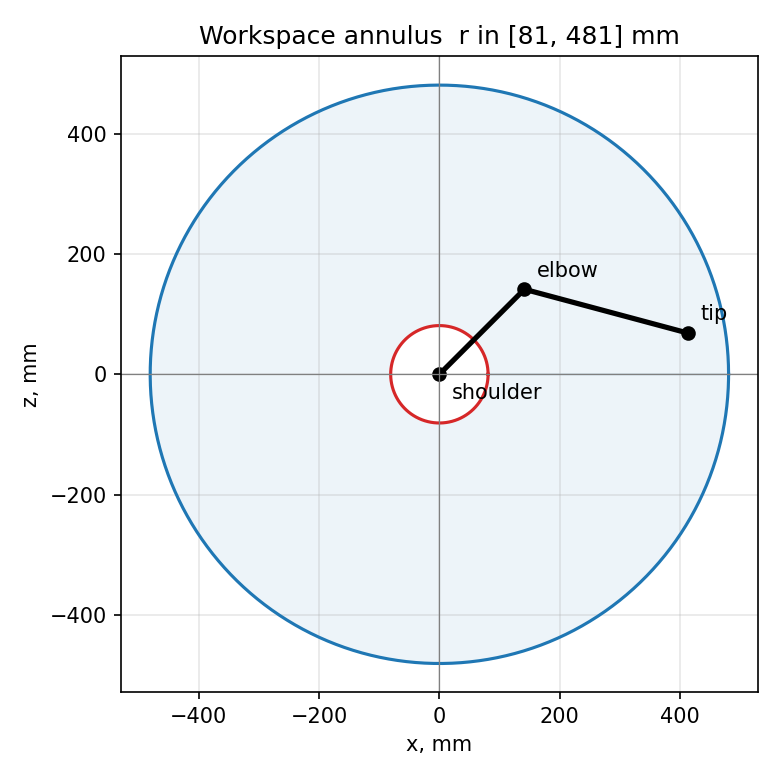
\includegraphics[width=0.55\textwidth]{fig_workspace.png}
\caption{Кольцевая рабочая зона $r\in[\,|L_1-L_2|,\,L_1+L_2]$ и пример позы.}
\end{figure}

\section{Суставные координаты и отсчёты энкодера}

Угол сустава передаётся на вал через волновой редуктор $N_i$; драйвер считает
$\mathrm{CPR}$ отсчётов на оборот вала (электронный редуктор драйвера $1{:}1$):
\begin{align}
\text{counts}_i&=\text{home}_i+\dir_i\cdot\frac{q_i-q_{0,i}}{2\pi}\,N_i\,\mathrm{CPR},\label{eq:jm1}\\
q_i&=q_{0,i}+\dir_i\cdot\frac{\text{counts}_i-\text{home}_i}{N_i\,\mathrm{CPR}}\,2\pi,\label{eq:jm2}
\end{align}
где $\dir_i\in\{+1,-1\}$~--- знак согласования фрейма с физикой; $\text{home}_i$~---
отсчёт в нулевой позе (абсолютный энкодер выдаёт произвольное число при
включении). Калиброванные значения: $\mathrm{CPR}=2^{23}=8\,388\,608$,
$N=(50,100)$, $\dir=(-1,-1)$.

\section{Планирование траектории}

Симметричный трапецеидальный профиль. Для пути $d\ge0$ при пределах $v_\text{m},
a_\text{m}$ минимальное время:
\begin{equation}
T=\begin{cases}
2\sqrt{d/a_\text{m}}, & d\le v_\text{m}^2/a_\text{m}\ (\text{треуг.}),\\[2pt]
d/v_\text{m}+v_\text{m}/a_\text{m}, & \text{иначе (трапеция).}
\end{cases}\label{eq:tmin}
\end{equation}
Оси \emph{синхронизируются}: общее время $T=\max_i T_i$; для заданного $T$
крейсерская скорость из $d=vT-v^2/a$:
\begin{equation}
v=\frac{aT-\sqrt{(aT)^2-4ad}}{2}.\label{eq:vcruise}
\end{equation}
Профиль положения ($t_a=v/a$):
\begin{equation}
s(t)=\begin{cases}
\tfrac12 a t^2, & 0\le t<t_a,\\
\tfrac12 a t_a^2+v(t-t_a), & t_a\le t<T-t_a,\\
d-\tfrac12 a (T-t)^2, & T-t_a\le t\le T.
\end{cases}\label{eq:profile}
\end{equation}

\begin{figure}[h]\centering
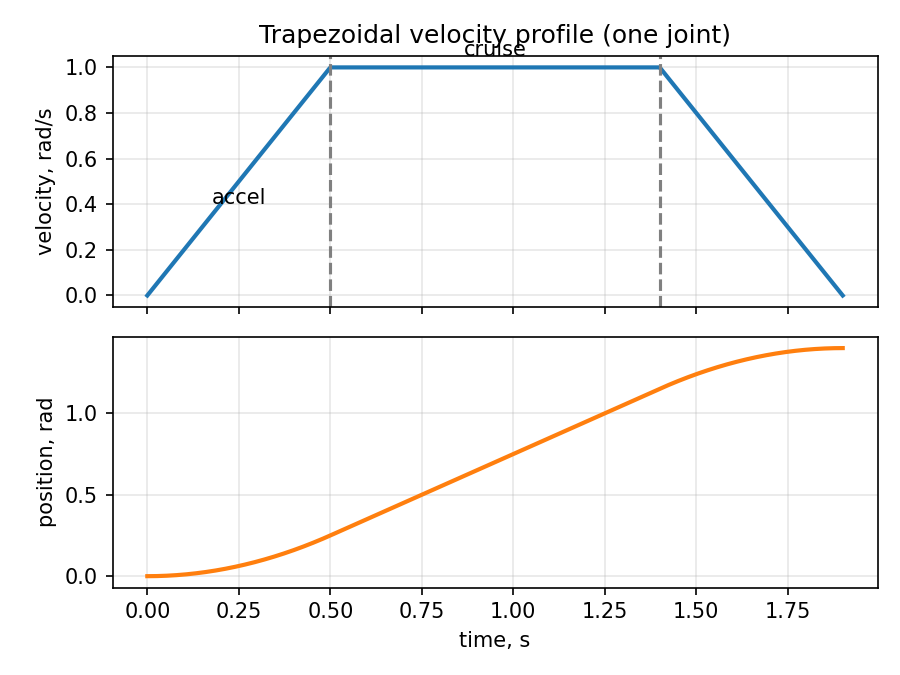
\includegraphics[width=0.7\textwidth]{fig_trapezoid.png}
\caption{Трапецеидальный профиль скорости и положения одного сустава.}
\end{figure}

\section{Шинный уровень: Cyclic Synchronous Position}

Приводы работают в CiA~402 mode~8 (CSP): хост каждые 4\,мс задаёт целевое
положение (\texttt{0x607A}), драйвер его отрабатывает; фактическое положение~---
\texttt{0x6064}, момент~--- \texttt{0x6077}. Защиты: захват цели по фактическому
положению при включении (иначе рывок к нулю); программное ограничение скорости
нарастания цели; ограничение момента объектами \texttt{0x60E0}/\texttt{0x60E1}
(на Y7 действует именно оно, а не \texttt{0x6072}).

\section{Момент, разложение и устранение трения}

Момент двигателя уравновешивает сумму, приведённую к валу через $N$ и КПД
$\eta$:
\begin{equation}
\tau_\text{м} N\eta=\tau_\text{ин}(q,\ddot q)+\tau_\text{кор}(q,\dot q)
+\tau_\text{грав}(q)+\tau_\text{пол}+\tau_\text{трен}(\dot q).\label{eq:balance}
\end{equation}
В квазистатике ($\dot q,\ddot q\approx0$) остаётся
$\tau_\text{м} N\eta\approx\tau_\text{нагр}+\tau_\text{трен}$, где
$\tau_\text{нагр}=\tau_\text{грав}+\tau_\text{пол}$.

\paragraph{Устранение трения.} Трение~--- нечётная функция скорости, нагрузка от
неё не зависит. Проходя одну позу медленно «туда» и «обратно»:
\begin{equation}
\tau_\text{нагр}=\tfrac12(\tau_\rightarrow+\tau_\leftarrow),\qquad
\tau_\text{трен}=\tfrac12(\tau_\rightarrow-\tau_\leftarrow).\label{eq:defric}
\end{equation}
В первом выражении кулоновское и вязкое трение взаимно сокращаются. Процедура
реализована как «проба»: медленный свип $\pm\Delta$ с усреднением момента по
участку постоянной скорости.

\begin{figure}[h]\centering
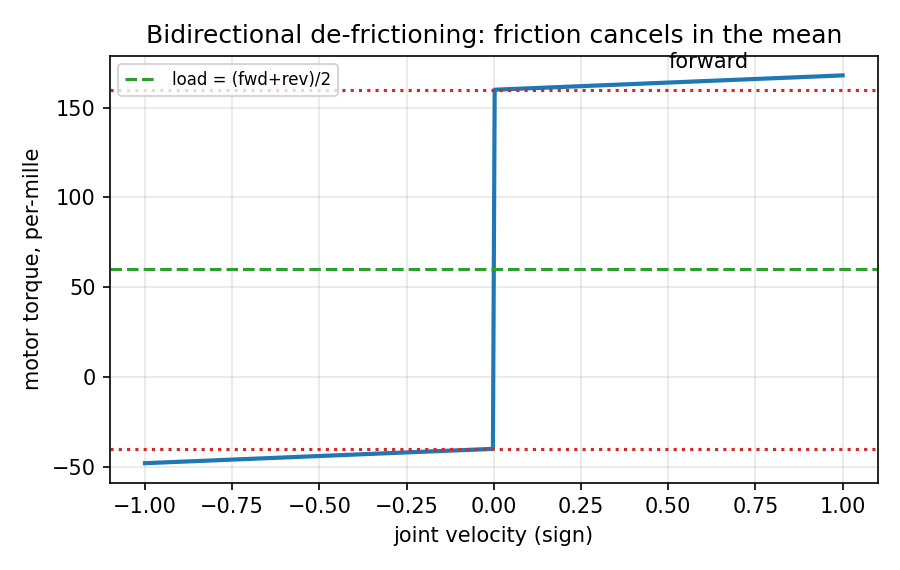
\includegraphics[width=0.62\textwidth]{fig_friction.png}
\caption{Двунаправленное усреднение: трение сдвигает момент на $\pm\tau_\text{трен}$,
среднее восстанавливает нагрузку.}
\end{figure}

\section{Идентификация модели статической нагрузки $G(q)$}

Момент силы тяжести в суставе $i$~--- сумма моментов весов дистальных масс на их
горизонтальные плечи:
\begin{equation}
\tau_{\text{грав},i}=g\sum_k m_k\,x_k(q).\label{eq:grav-phys}
\end{equation}
Подстановка горизонтальных координат из \eqref{eq:fk} даёт
\begin{equation}
\tau_{\text{грав},0}=A\cos q_0+B\cos(q_0+q_1),\qquad
\tau_{\text{грав},1}=B\cos(q_0+q_1).\label{eq:grav-form}
\end{equation}
Рабочая форма (линейная по параметрам; члены $\sin$~--- смещение центра масс,
константа~--- сдвиг датчика), отдельно по осям и \emph{в единицах момента
мотора}:
\begin{align}
m_0(q)&=c_{00}\cos q_0+c_{01}\sin q_0+c_{02}\cos(q_0{+}q_1)+c_{03}\sin(q_0{+}q_1)+c_{04},\label{eq:g0}\\
m_1(q)&=c_{10}\cos(q_0{+}q_1)+c_{11}\sin(q_0{+}q_1)+c_{12}.\label{eq:g1}
\end{align}
Подгонка под измеренный момент сворачивает неизвестные $N,\eta$ и масштаб
«\permil{} на Н$\cdot$мм» в коэффициенты $c_{ij}$; каждая ось остаётся в своих
единицах, что согласуется с компенсацией. Коэффициенты находятся МНК по набору
поз $q^{(k)}$ с измеренной по \eqref{eq:defric} нагрузкой:
\begin{equation}
\Phi_j c_j=y_j,\qquad c_j=(\Phi_j^\top\Phi_j)^{-1}\Phi_j^\top y_j.\label{eq:lsq}
\end{equation}
Сбор данных (\texttt{gravcal}): автономный обход безопасной сетки поз (в пределах
суставов и выше декартова «пола», чтобы не задеть стол), проба в каждой.

\begin{figure}[h]\centering
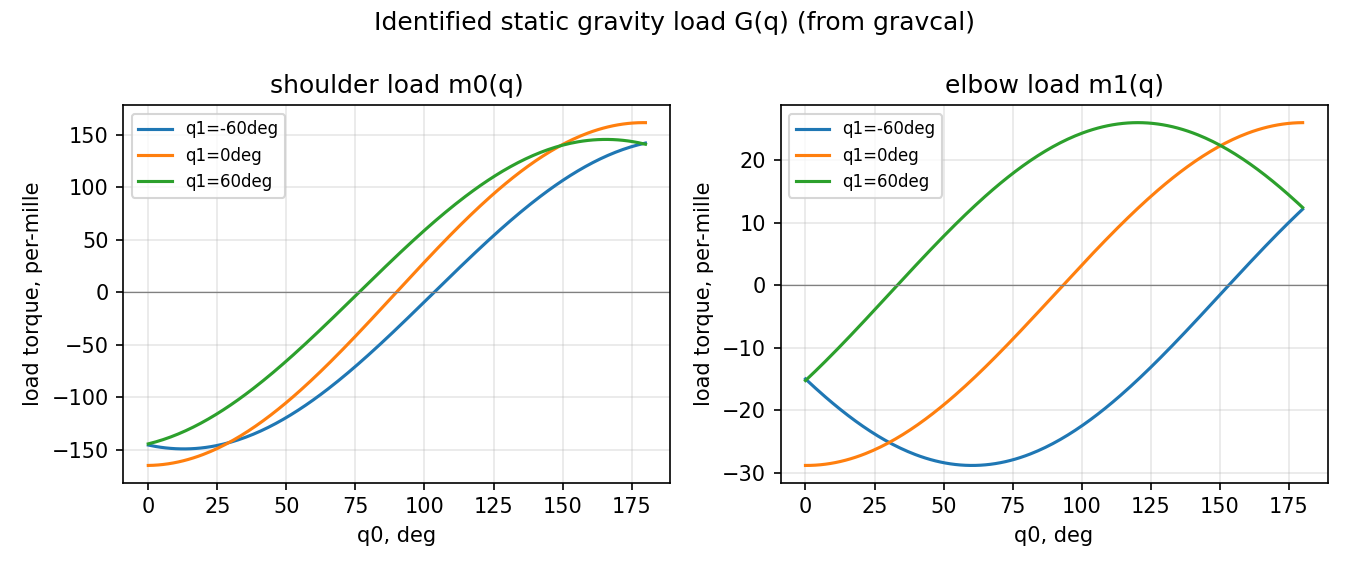
\includegraphics[width=0.95\textwidth]{fig_gravity.png}
\caption{Идентифицированный момент нагрузки $G(q)$: плечо и локоть.}
\end{figure}

\section{Модель упругой деформации}

Упругий элемент между валом и звеном (податливость редуктора $+$ изгиб звена)
моделируется крутильной пружиной с эффективной жёсткостью $K_{\text{эф},i}$:
\begin{equation}
\theta_\text{звено}=\theta_\text{мотор}-\frac{\tau_\text{нагр}}{K_\text{эф}}.\label{eq:spring}
\end{equation}
Звено отстаёт от вала на $\delta=\tau_\text{нагр}/K_\text{эф}$; так как датчик
меряет $\theta_\text{мотор}$, деформация невидима и оценивается по
\eqref{eq:spring}. «Лумпированная» жёсткость объединяет податливость редуктора и
изгиб звена в один коэффициент на сустав.

\section{Идентификация жёсткости $K_\text{эф}$}

Индикатор крепится только к кончику, а деформируются обе оси. Вертикальный прогиб
кончика через якобиан:
\begin{equation}
\Delta z=J_0\delta_0+J_1\delta_1,\quad
J_0=\frac{\partial z}{\partial q_0}=x_\text{конч},\quad
J_1=\frac{\partial z}{\partial q_1}=L_2\cos(q_0+q_1).\label{eq:jac}
\end{equation}
Известный груз даёт прирост нагрузки $\Delta m_i$ (проба «с грузом» минус $G(q)$)
и деформацию $\delta_i=\Delta m_i/K_i$. Тогда
\begin{equation}
\Delta z=(J_0\Delta m_0)\frac{1}{K_0}+(J_1\Delta m_1)\frac{1}{K_1},\label{eq:stiff-lsq}
\end{equation}
линейно по $1/K_i$. По нескольким позам МНК разделяет обе жёсткости. Всё в
\permil{}, поэтому $K_i$ получаются в \permil{}/рад и стыкуются с компенсацией.

\paragraph{Наблюдаемость.} Разделение возможно лишь при линейно независимых
столбцах $(J_i\Delta m_i)^{(k)}$. Позы с $q_0+q_1=90^\circ$ дают $J_1=0$ и не
несут информации о $K_1$; позы подбираются максимизацией минимального
сингулярного числа нормированной матрицы якобианов.

\begin{figure}[h]\centering
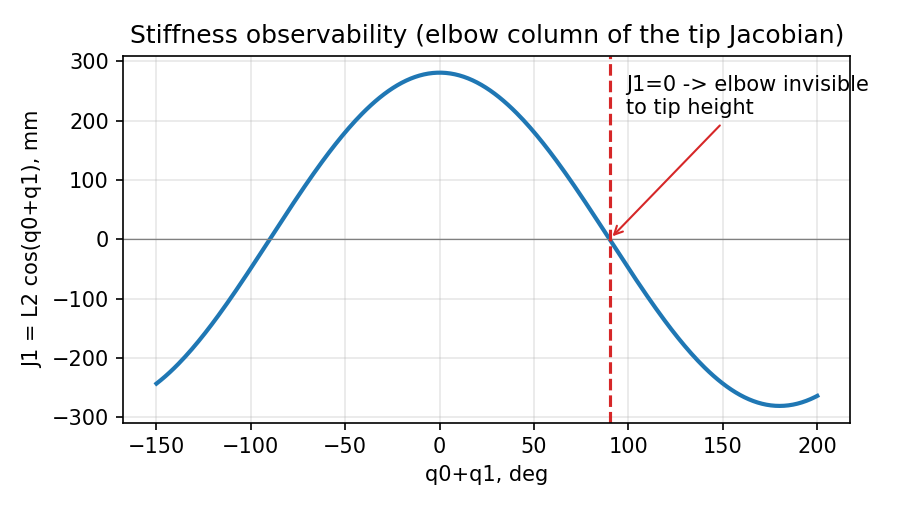
\includegraphics[width=0.62\textwidth]{fig_observability.png}
\caption{$J_1=L_2\cos(q_0+q_1)$ обращается в ноль при $q_0+q_1=90^\circ$.}
\end{figure}

\section{Компенсация деформации}

Предсказанная деформация в целевой позе и командный угол:
\begin{equation}
\delta_i(q_\text{ц})=\frac{G_i(q_\text{ц})}{K_{\text{эф},i}},\qquad
q_{\text{кмд},i}=q_{\text{ц},i}+\delta_i(q_\text{ц}).\label{eq:comp}
\end{equation}
Из \eqref{eq:spring}: чтобы звено село в $q_\text{ц}$, вал выводят «дальше» на
величину деформации. Это упреждение от модели~--- живой момент в путь не входит,
полоса трения не вносит шум. Знаки согласованы (общая конвенция \permil{} и
$\dir$) и подлежат проверке на стенде: при включённой компенсации прогиб кончика
в нагруженной позе должен уменьшаться.

\begin{figure}[h]\centering
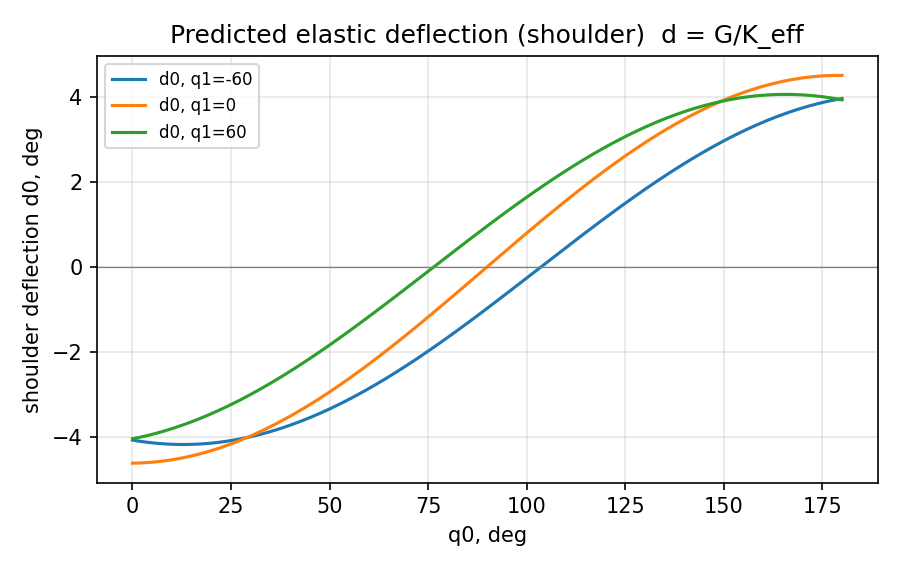
\includegraphics[width=0.62\textwidth]{fig_deflection.png}
\caption{Предсказанная деформация плеча $\delta_0=G_0/K_\text{эф,0}$~--- величина
поправки.}
\end{figure}

\section{Экспериментальные результаты}

\subsection{Калибровка геометрии и привода}
\begin{table}[h]\centering\small
\begin{tabular}{@{}lll@{}}\toprule
Параметр & Метод & Результат\\\midrule
$\mathrm{CPR}$ & «1 оборот вала» & $2^{23}=8\,388\,608$ отсч/об\\
$N$ & «поворот на угол» & $(50,100)$ — вдвое меньше номинала (ступень 2:1)\\
$\dir$ & толчковый тест & $(-1,-1)$\\
Лимиты & механика & $q_0\in[-1^\circ,181^\circ]$; $q_1=\pm110^\circ$\\\bottomrule
\end{tabular}
\caption{Результаты калибровки геометрии и привода.}
\end{table}

\subsection{Модель $G(q)$ (19 поз)}
\begin{table}[h]\centering\small
\begin{tabular}{@{}llll@{}}\toprule
Ось & Диапазон нагрузки & СКО остатка & Макс. остаток\\\midrule
Плечо & $\pm164\permil$ & $1.22\permil$ & $2.36\permil$\\
Локоть & $\pm29\permil$ & $0.80\permil$ & $1.75\permil$\\\bottomrule
\end{tabular}
\caption{Качество подгонки $G(q)$ (СКО $<1\%$ от диапазона).}
\end{table}
Коэффициенты (\permil{}): плечо $[-123.2,\,1.50,\,-39.99,\,0.65,\,-1.82]$;
локоть $[-27.41,\,-0.15,\,-1.41]$. Доминируют косинусные члены, как в
\eqref{eq:grav-form}.

\subsection{Трение и жёсткость}
\begin{table}[h]\centering\small
\begin{tabular}{@{}lll@{}}\toprule
Ось & $|\tau_\text{трен}|$ (среднее) & $K_\text{эф}$, \permil{}/рад\\\midrule
Плечо & $\approx103\permil$ ($\approx10\%$) & $\approx2050$ (измерено)\\
Локоть & $\approx49\permil$ ($\approx5\%$) & $\approx4000$ (провизорно)\\\bottomrule
\end{tabular}
\caption{Трение почти постоянно по позам; жёсткость локтя требует повторной
калибровки.}
\end{table}
Для цели $(300,150)\mm$ ($q\approx(83^\circ,-93^\circ)$): $G\approx(-54,-28)\permil$,
поправка $\delta\approx(-1.5^\circ,-0.4^\circ)$.

\section{Допущения и ограничения}
\begin{enumerate}\itemsep2pt
\item Квазистатика: инерционные/кориолисовы члены не компенсируются.
\item Линейная жёсткость $\delta\propto\tau$; вязкоупругость и ползучесть
полимера не учтены.
\item Деформация не измеряется, а оценивается по модели~--- точность ограничена
качеством калибровки.
\item Лумпированная модель на сустав (приближение распределённого изгиба).
\item Полезная нагрузка входит в те же гармоники, что вес звена~2; неизвестная
нагрузка может оцениваться отдельным наблюдателем (задел на будущее).
\end{enumerate}

\end{document}
